\documentclass[11pt]{amsart}

\date{\today}

\usepackage[margin=1in]{geometry}
\usepackage{tikz}
\usetikzlibrary{calc, shapes.geometric, positioning, shapes, snakes, arrows, shapes, patterns}
\usepackage{setspace}
\usepackage{amsmath}
\usepackage{amsthm}
\usepackage{amssymb}
\usepackage{mathtools}
\usepackage{mathdots}
\usepackage{enumitem}
\usepackage{graphicx}
\usepackage{caption}
\usepackage[labelformat=simple,labelfont={}]{subcaption}
\usepackage{color}
\definecolor{darkblue}{rgb}{0, 0, .6}
\usepackage{hyperref}
\hypersetup{
	colorlinks=true,
	linkcolor=darkblue,
	anchorcolor=darkblue,
	citecolor=darkblue,
	pagecolor=darkblue,
	urlcolor=darkblue,
	pdftitle=darkblue,
	pdfauthor=darkblue
}

\newtheorem{theorem}{Theorem}[subsection]
\newtheorem{lemma}[theorem]{Lemma}
\newtheorem{claim}[theorem]{Claim}
\newtheorem{corollary}[theorem]{Corollary}
\newtheorem{proposition}[theorem]{Proposition}
\newtheorem{conjecture}[theorem]{Conjecture}

\theoremstyle{definition} 
\newtheorem{definition}[theorem]{Definition}
\newtheorem{example}[theorem]{Example}
\newtheorem{remark}[theorem]{Remark}

\numberwithin{equation}{section}

\newcommand{\Z}{\mathbb{Z}}
\newcommand{\N}{\mathbb{N}}
\newcommand{\A}{\mathcal{A}}
\newcommand{\C}{\widetilde{C}}
\renewcommand{\O}{\mathcal{O}}
\newcommand{\E}{\mathcal{E}}
\newcommand{\z}{\mathsf{z}}
\newcommand{\x}{\mathsf{x}}
\newcommand{\y}{\mathsf{y}}
\renewcommand{\u}{\mathsf{u}}
\renewcommand{\v}{\mathsf{v}}
\newcommand{\wtri}{\vartriangle}
\newcommand{\btri}{\blacktriangle}
\renewcommand{\a}{\mathbf{a}}
\DeclareMathOperator{\TL}{TL}
\DeclareMathOperator{\DTL}{\mathbb{D}TL}
\renewcommand{\P}{\mathcal{P}}
\newcommand{\V}{\mathcal{V}}
\newcommand{\D}{\mathbb{D}}
\newcommand{\B}{\mathbf{B}}
\newcommand{\I}{\mathcal{I}}
\newcommand{\Diag}{\mathcal{D}}
\newcommand{\wcirc}{\circ}
\newcommand{\wbox}{\square}
\newcommand{\bcirc}{\bullet}
\newcommand{\bbox}{\blacksquare}
\newcommand{\supp}{\mathrm{supp}}
\renewcommand{\L}{\mathcal{L}}
\newcommand{\R}{\mathcal{R}}
\renewcommand{\(}{\left(}
\renewcommand{\)}{\right)}
\newcommand{\w}{\mathsf{w}}
\renewcommand{\H}{\mathcal{H}}
\DeclareMathOperator{\FC}{FC}
\renewcommand{\r}{\mathbf{r}}
\newcommand{\Sup}{\textrm{Sup}}

\renewcommand\arraystretch{1.5}
\renewcommand\thesubfigure{(\alph{subfigure})}

\definecolor{purple}{RGB}{153,51,255}
\definecolor{darkblue}{RGB}{0,0,255}

%%% TikZ for Heaps %%%

%For Heaps. command of the form \heapblock{a}{b}{c} where a is the index of the generator, b is the level in the heap (starting at the bottom), c is the label

\newcommand\xxaxis{0}
\newcommand\yyaxis{90}

\newcommand\heapblock[3]{\fill[draw=black, fill=gray!30, rounded corners, line width=1.1pt, shift={(\xxaxis:#1)},shift={(\yyaxis:#2)}] (-1,-0.5) rectangle (1,0.5);\node at (#1,#2) {$#3$};}

\newcommand\heapblank[2]{\fill[fill=white, dotted, draw=black, line width=1.1pt, rounded corners, shift={(\xxaxis:#1)},shift={(\yyaxis:#2)}] (-1,-0.5) rectangle (1,0.5);}

\newcommand\nsq[3]{\fill[fill=cyan!30, draw=black, rounded corners, line width=1pt, shift={(\xxaxis:#1)},shift={(\yyaxis:#2)}] (0,0) -- (2,0) -- (2,-2) -- (0,-2) --cycle;\node at (#1+1,#2-1) {$#3$};}

%%% TikZ for Diagrams %%%

% loops
\newcommand\dlp[2]{
\fill[fill=white, draw=black] (#1,#2) ellipse (16pt and 8pt);
\draw[fill=black, xshift=-16pt] (#1,#2) circle (2.8pt);
}

\newcommand\lp[2]{\draw[out=90,in=90] (#1,#2) to (#1 + 1,#2) [out=-90,in=-90] to (#1,#2);}

\newcommand\blacktrilp[2]{\draw[out=90,in=90] (#1,#2) to node[blacktri, pos=0.5]{} (#1 + 1,#2) [out=-90,in=-90] to (#1,#2);}

\newcommand\whitetrilp[2]{\draw[out=90,in=90] (#1,#2) to node[whitetri, pos=0.5]{} (#1 + 1,#2) [out=-90,in=-90] to (#1,#2);}

\newcommand\blackwhitetrilp[2]{\draw[out=90,in=90] (#1,#2) to node[blacktri, pos=0.5]{} (#1 +1,#2) [out=-90,in=-90] to node[whitetri, pos=0.5]{} (#1,#2);}

%%%%%%%%%% begin document %%%%%%%%%%%

\begin{document}

\tikzstyle{blacktri} = [draw=black, fill=black, rotate=-90, sloped, regular polygon, regular polygon sides=3, inner sep=1.3pt]
\tikzstyle{whitetri} = [draw=black, fill=white, rotate=-90, sloped, regular polygon, regular polygon sides=3, inner sep=1.3pt]
\tikzstyle{blackcirc} = [draw=black, fill=black, shape=circle, inner sep=1.8pt]
\tikzstyle{whitecirc} = [draw=black, fill=white, shape=circle, inner sep=1.8pt]

\title[T-avoiding elements in Coxeter groups of type $A$ and $B$]{T-avoiding elements in Coxeter groups of type $A$ and $B$}

\author[D.C.~Ernst]{Dana C.~Ernst}
\address{Department of Mathematics and Statistics, Northern Arizona University, Flagstaff, AZ 86011}
\email{\url{dana.ernst@nau.edu}}
\urladdr{\url{http://danaernst.com}}

\author[T.M.~Laird]{Taryn M.~Laird}
\address{Department of Mathematics and Statistics, Northern Arizona University, Flagstaff, AZ 86011}
\email{\url{tml94@nau.edu}}

\subjclass[2000]{20F55, 20C08, 57M15}
\keywords{diagram algebra, Temperley--Lieb algebra, Coxeter groups, heaps}

%%%%%%%%%% abstract %%%%%%%%%%%

\begin{abstract}
Abstract Stuff Here
\end{abstract}

\maketitle

%%%%%%%  introduction %%%%%%%%%%%%%

\begin{section}{Introduction}\label{sec:intro}
TO DO LAST
%The (type $A$) Temperley--Lieb algebra $\TL(A)$, invented by H.N.V.~Temperley and E.H.~Lieb in 1971~\cite{Temperley1971}, is a finite dimensional associative algebra which first arose in the context of statistical mechanics.
%
%In 1987, V.F.R.~Jones showed that $\TL(A)$ occurs naturally as a quotient of the type $A$ Hecke algebra, $\H(A)$~\cite{Jones1999}.  If $(W,S)$ is Coxeter system of type $\Gamma$, the associated Hecke algebra $\H(\Gamma)$ is an algebra with a basis given by $\{T_w\mid w \in W\}$ and relations that deform the relations of $W$ by a parameter $q$. The realization of the Temperley--Lieb algebra as a Hecke algebra quotient was generalized by J.J.~Graham in~\cite{Graham1995} to the case of an arbitrary Coxeter system.  %In Section~\ref{subsec:TL-algebras}, we define the generalized Temperley--Lieb algebra of type $\C_{n}$, denoted $\TL(\C_{n})$, and describe a special basis, called the monomial basis, which is indexed by the fully commutative elements (defined in Section~\ref{subsec:FC}) of the underlying Coxeter group.
%
%%Moreover, studying these generalized Temperley--Lieb algebras often provides a gateway to understanding the Kazhdan--Lusztig theory of the associated Hecke algebra.  Loosely speaking, $\TL(\Gamma)$ retains some of the relevant structure of $\H(\Gamma)$, yet is small enough that computation of the leading coefficients of the notoriously difficult to compute Kazhdan--Lusztig polynomials is often much simpler.
%
%Section~\ref{sec:prelim} of this paper is concerned with introducing the necessary notation and terminology of Coxeter groups, fully commutative elements, and heaps.  The concept of a heap introduced in Section~\ref{subsec:heaps} will be our main tool for visualizing combinatorial arguments required to prove several technical lemmas appearing in Section~\ref{subsec:prep lemmas}.  
%%In Section~\ref{sec:combinatorics}, we study some of the combinatorics of Coxeter groups of types $B$ and $\C$.  In particular, we introduce weak star reductions and the type I, type II, and non-cancellable elements of a Coxeter group of type $\C$, as well as establish several intermediate results.  The necessary background on generalized Temperley--Lieb algebras (in the sense of Graham) is summarized in Section~\ref{sec:gen TL-algebras}.  
%Lastly, in Section~\ref{sec:closing}, we discuss the implications of our results and future research.

\end{section}

%%%%%%%  preliminaries %%%%%%%%%%%%%

\begin{section}{Preliminaries}\label{sec:prelim}

%%%%%%%%%%%%% Coxeter groups %%%%%%%%%%%%

\begin{subsection}{Coxeter groups}\label{subsec:coxeter groups}

A \emph{Coxeter system} is pair $(W,S)$ consisting of a distinguished (finite) set $S$ of generating involutions and a group $W$, called a \emph{Coxeter group}, with presentation
\[
W = \langle S \mid (st)^{m(s, t)} = e \text{ for } m(s, t) < \infty \rangle,
\]
where $e$ is the identity, $m(s,t) = 1$ if and only if $s = t$, and $m(s,t) = m(t,s)$. It turns out that the elements of $S$ are distinct as group elements, and that $m(s, t)$ is the order of $st$.  Since the elements of $S$ have order two, the relation $(st)^{m(s,t)} = e$ can be written as
\[
\underbrace{sts \cdots}_{m(s,t)} = \underbrace{tst \cdots}_{m(s,t)}
\]
with $m(s,t) \geq 2$ factors.

Given a Coxeter system $(W,S)$, a word $s_{x_1}s_{x_2}\cdots s_{x_m}$ in the free monoid $S^*$ is called an \emph{expression} for $w\in W$ if it is equal to $w$ when considered as a group element. If $m$ is minimal among all expressions for $w$, the corresponding word is called a \emph{reduced expression} for $w$. In this case, we define the \emph{length} of $w$ to be $\ell(w)=m$. Each element $w \in W$ can have several different reduced expressions that represent it.  If we wish to emphasize a fixed, possibly reduced, expression for $w\in W$, we represent it  in \textsf{sans serif} font, say $\w=s_{x_1}s_{x_2}\cdots s_{x_m}$, where each $s_{x_i} \in S$.  A product $w_{1}w_{2}\cdots w_{r}$ with $w_{i} \in W$ is called \emph{reduced} if $\ell(w_{1}w_{2}\cdots w_{r})=\sum \ell(w_{i})$. {\color{red}We may not need reduced product.}

Matsumoto's Theorem~\cite[Theorem 1.2.2]{Geck2000} states that if $w \in W$, then every reduced expression for $w$ can be obtained from any other by applying a sequence of \emph{braid moves} of the form 
\[
{\underbrace{sts \cdots }_{m(s,t)} } \mapsto {\underbrace{tst \cdots}_{m(s,t)}}
\]
where $s,t \in S$ and each factor in the move has $m(s,t)$ letters.  %The \emph{support} of an element $w \in W$, denoted $\supp(w)$, is the set of all generators appearing in any reduced expression for $w$ (which is well-defined by Matsumoto's Theorem).

%Given a reduced expression $\w$ for $w \in W$, we define a \emph{subexpression} of $\w$ to be any subsequence of $\w$. We will refer to a subexpression consisting of a string of consecutive symbols from $\w$ as a \emph{subword} of $\w$.

The sets $\L(w)=\{s \in S\mid \ell(sw) < \ell(w)\}$ and $\R(w)=\{s \in S\mid \ell(ws) < \ell(w)\}$ are called the \emph{left} and \emph{right descent sets} of $w$, respectively.  It turns out that $s \in \L(w)$ (respectively, $\R(w)$) if and only if $w$ has a reduced expression beginning (respectively, ending) with $s$.

Given a Coxeter system $(W,S)$, the associated \emph{Coxeter graph} is the graph $\Gamma$ with vertex set $S$ and edges $\{s,t\}$ labeled with $m(s,t)$ for all $m(s,t)\geq 3$.  If $m(s,t)=3$, it is customary to leave the corresponding edge unlabeled.  Given a Coxeter graph $\Gamma$, we can uniquely reconstruct the corresponding Coxeter system $(W,S)$.  In this case, we say that $(W,S)$, or just $W$, is of type $\Gamma$. If $(W,S)$ is of type $\Gamma$, for emphasis, we may write $(W,S)$ as $(W(\Gamma),S(\Gamma))$.  Note that generators $s$ and $t$ are connected by an edge in the Coxeter graph $\Gamma$ if and only if $s$ and $t$ do not commute~\cite{Humphreys1990}.

The main focus of this paper will be the Coxeter systems of types $A_n$ and $B_n$, which are defined by the Coxeter graphs in Figures~\ref{fig:typeA} and \ref{fig:typeB}, respectively, where $n\geq 2$.

\begin{figure}[!ht]
\subcaptionbox{$A_n$\label{fig:typeA}}[.4\textwidth]{
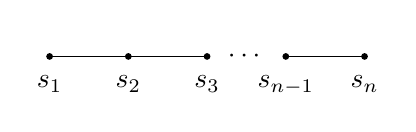
\begin{tikzpicture}
\draw[fill=black] \foreach \x in {1,2,3,4,5} {(\x,10) circle (1pt)};
\draw \foreach \x in {1,2,3} {(\x,10) node[label=below:$s_{\x}$]{}};
\draw (1.5,10) node[label=above:$$]{};
\draw {(4,10) node[label=below:$s_{n-1}$]{}};
\draw {(5,10) node[label=below:$s_{n}$]{}};
\draw {(3.5,10) node[]{$\cdots$}};
\draw[-] (1,10) -- (3,10);
\draw[-] (4,10) -- (5,10);
\end{tikzpicture}
}
\subcaptionbox{$B_n$\label{fig:typeB}}[.4\textwidth]{
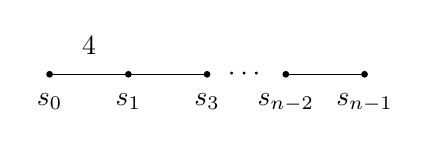
\begin{tikzpicture}
\draw[fill=black] \foreach \x in {1,2,3,4,5} {(\x,10) circle (1pt)};
%\draw \foreach \x in {1,2,3} {(\x,10) node[label=below:$s_{\x}$]{}};
\draw (1.5,10) node[label=above:$4$]{};
\draw {(1,10) node[label=below:$s_{0}$]{}};
\draw {(2,10) node[label=below:$s_{1}$]{}};
\draw {(3,10) node[label=below:$s_{3}$]{}};
\draw {(4,10) node[label=below:$s_{n-2}$]{}};
\draw {(5,10) node[label=below:$s_{n-1}$]{}};
\draw {(3.5,10) node[]{$\cdots$}};
\draw[-] (1,10) -- (3,10);
\draw[-] (4,10) -- (5,10);
\end{tikzpicture}
}
\caption{Coxeter graphs corresponding to Coxeter systems of type $A_{n}$ and $B_n$.}\label{fig:CoxeterGraphs}
\end{figure}

%We can obtain $W(B_{n})$ from $W(\C_{n})$ by removing the generator $s_{n+1}$ and the corresponding relations~\cite[Chapter 5]{Humphreys1990}.  We also obtain a Coxeter group of type $B$ if we remove the generator $s_{1}$ and the corresponding relations.  To distinguish these two cases, we let $W(B_{n})$ denote the subgroup of $W(\C_{n})$ generated by $\{s_{1}, s_{2}, \dots, s_{n}\}$ and we let $W(B'_{n})$ denote the subgroup of $W(\C_{n})$ generated by $\{s_{2}, s_{3}, \dots, s_{n+1}\}$.  It is well known that $W(\C_{n})$ is an infinite Coxeter group while $W(B_{n})$ and $W(B'_{n})$ are both finite~\cite[Chapters 2 and 6]{Humphreys1990}.

\end{subsection}

%%%%%%%%  FC elements %%%%%%%%%%%%%

\begin{subsection}{Fully commutative elements}\label{subsec:FC}

Let $(W,S)$ be a Coxeter system of type $\Gamma$ and let $w \in W$. Following Stembridge~\cite{Stembridge1996}, we define a relation $\sim$ on the set of reduced expressions for $w$.  Let $\w$ and $\w'$ be two reduced expressions for $w$.  We define $\w \sim \w'$ if we can obtain $\w'$ from $\w$ by applying a single commutation move of the form $st \mapsto ts$, where $m(s,t)=2$.  Now, define the equivalence relation $\approx$ by taking the reflexive transitive closure of $\sim$.  Each equivalence class under $\approx$ is called a \emph{commutation class}. If $w$ has a single commutation class, then we say that $w$ is \emph{fully commutative} (FC).  According to a result in~\cite{Stembridge1996}, an element $w$ is FC if and only if no reduced expression for $w$ contains a subword of the form $sts \cdots$ of length $m(s,t) \geq 3$.  The set of FC elements of the Coxeter system $(W,S)$ of type $\Gamma$ is denoted by $\FC(\Gamma)$, or possibly $\FC(W)$.

\begin{remark}\label{rem:illegal convex chains}
The elements of $\FC(\C_{n})$ are precisely those whose reduced expressions avoid consecutive subwords of the following types:
\begin{enumerate}
\item $s_{i}s_{j}s_{i}$ for $|i-j|=1$ and $1< i,j < n+1$;
\item $s_{i}s_{j}s_{i}s_{j}$ for $\{i,j\}=\{1,2\}$ or $\{n,n+1\}$.
\end{enumerate}
Note that the FC elements of $W(B_{n})$ and $W(B'_{n})$ avoid the respective subwords above.
\end{remark}

In~\cite{Stembridge1996}, Stembridge classified the Coxeter groups that contain a finite number of FC elements.  According to~\cite[Theorem 5.1]{Stembridge1996}, $W(\C_{n})$ contains an infinite number of FC elements, while $W(B_{n})$ (and hence $W(B'_n)$) contains finitely many.  There are examples of infinite Coxeter groups that contain a finite number of FC elements (e.g., $W(E_n$) is infinite for $n\geq 9$, but contains only finitely many FC elements~\cite[Theorem 5.1]{Stembridge1996}).

\end{subsection}

%%%%%%%%%%%%%%%%%%%%%

\begin{subsection}{Heaps}\label{subsec:heaps}

Every reduced expression can be associated with a partially ordered set called a heap that will allow us to visualize a reduced expression  while preserving the essential information about the relations among the generators.  The theory of heaps was introduced in~\cite{Viennot1986} by Viennot and visually capture the combinatorial structure of the Cartier--Foata monoid of~\cite{Cartier1969}.  
In~\cite{Stembridge1996} and~\cite{Stembridge1998}, Stembridge studied heaps in the context of fully commutative elements, which is our motivation here.  
In this section, we mimic the development found in~\cite{Billey2007},~\cite{Ernst2010}, and~\cite{Stembridge1996}.

Let $(W,S)$ be a Coxeter system.  Suppose $\w = s_{x_1} \cdots s_{x_r}$ is a fixed reduced expression for $w \in W$.  As in~\cite{Stembridge1996}, we define a partial ordering on the indices $\{1, \dots, r\}$ by the transitive closure of the relation $\lessdot$ defined via $j \lessdot i$ if $i < j$ and $s_{x_i}$ and $s_{x_j}$ do not commute.  In particular, since $\w$ is reduced, $j \lessdot i$ if $i < j$ and $s_{x_i} = s_{x_j}$ by transitivity.  This partial order is referred to as the \emph{heap} of $\w$, where $i$ is labeled by $s_{x_i}$  Note that for simplicity, we are omitting the labels of the underlying poset but retaining the labels of the corresponding generators.

It follows from~\cite[Proposition 2.2]{Stembridge1996} that heaps are well-defined up to commutativity class.  That is, if $\w$ and $\w'$ are two reduced expressions for $w \in W$ that are in the same commutativity class, then the heaps of $\w$ and $\w'$ are equal.  
In particular, if $w$ is FC, then it has a single commutativity class, and so there is a unique heap associated to $w$.


\begin{example}\label{ex:first heap}
Let $\w = s_3 s_5 s_2 s_4 s_6 s_1 s_5 s_2$ be a reduced expression for $w \in (\A_{6})$.  We see that $\w$ is indexed by $\{1, 2, 3, 4, 5\}$.  As an example, $3 \lessdot 2$ since $2 < 3$ and the second and third generators do not commute.  The labeled Hasse diagram for the heap poset of $w$ is shown in Figure~\ref{fig:hasse}.
\end{example}

\begin{figure}[!ht]
\subcaptionbox{\label{fig:hasse}}[.4\textwidth]{ 
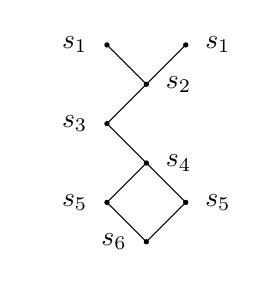
\begin{tikzpicture}[scale=0.5]
\draw [fill=black] (5,6) circle (1.5pt);
\draw (5,6) node[label=right:$s_1$]{};
\draw [fill=black] (3,6) circle (1.5pt);
\draw (3,6) node[label=left:$s_1$]{};
\draw [fill=black] (5,2) circle (1.5pt);
\draw (5,2) node[label=right:$s_5$]{};
\draw [fill=black] (4,5) circle (1.5pt);
\draw (4,5) node[label=right:$s_2$]{};
\draw [fill=black] (4,3) circle (1.5pt);
\draw (4,3) node[label=right:$s_4$]{};
\draw [fill=black] (4,1) circle (1.5pt);
\draw (4,1) node[label=left:$s_6$]{};
\draw [fill=black] (3,4) circle (1.5pt);
\draw (3,4) node[label=left:$s_3$]{};
\draw [fill=black] (3,2) circle (1.5pt);
\draw (3,2) node[label=left:$s_5$]{};
\draw [color=white] (1,.5) circle (0pt);
\draw (3,6)--(4,5)--(5,6)--(3,4)--(4,3)--(5,2)--(4,1)--(3,2)--(4,3);
\end{tikzpicture}
}
\subcaptionbox{\label{fig:first heap}}[.4\textwidth]{
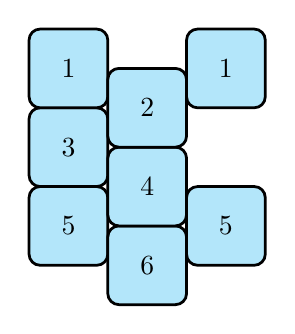
\begin{tikzpicture}[scale=0.5]
%\heapblock{5}{4}{s_5};
%\heapblock{3}{4}{s_3};
%\heapblock{6}{3}{s_6};
%\heapblock{4}{3}{s_4};
%\heapblock{2}{3}{s_2};
%\heapblock{5}{2}{s_5};
%\heapblock{1}{2}{s_1};
%\heapblock{2}{1}{s_2};

\nsq{0}{0}{5};
\nsq{0}{2}{3};
\nsq{0}{4}{1};
\nsq{2}{-1}{6};
\nsq{2}{1}{4};
\nsq{2}{3}{2};
\nsq{4}{0}{5};
\nsq{4}{4}{1};

\end{tikzpicture}
}
\caption{The labeled Hasse diagram and a possible lattice point representation for the heap of an element from $(\C_5)$.}
\end{figure}

Let $\w$ be a fixed reduced expression for $w \in W(\A_{n})$.  As in~\cite{Billey2007} and~\cite{Ernst2010}, we will represent a heap for $\w$ as a set of lattice points embedded in $\{1,2,\ldots,n+1\} \times \mathbb{N}$.  To do so, we assign coordinates (not unique) $(x,y) \in \{1,2,\ldots, n+1\} \times \mathbb{N}$ to each entry of the labeled Hasse diagram for the heap of $\w$ in such a way that:
\begin{enumerate}
\item an entry with coordinates $(x,y)$ is labeled $s_i$ in the heap if and only if $x = i$; 
\item an entry with coordinates $(x,y)$ is greater than an entry with coordinates $(x',y')$ in the heap if and only if $y > y'$.
\end{enumerate}
%If we change the heaps we need to fix the paragraph here. 
Recall that a finite poset is determined by its covering relations.  In the case of a Coxeter group of type $\A_{n}$ (and any straight line Coxeter graph), it follows from the definition that $(x,y)$ covers $(x',y')$ in the heap if and only if $x = x' \pm 1$, $y > y'$, and there are no entries $(x'', y'')$ such that $x'' \in \{x, x'\}$ and $y'< y'' < y$.  This implies that we can completely reconstruct the edges of the Hasse diagram and the corresponding heap poset from a lattice point representation. The lattice point representation of a heap allows us to visualize potentially cumbersome arguments.  In this case our heaps correspond to a left version of~\cite{Billey2007} and several other papers.  That is, in this paper entries at the left of a heap correspond to generators occurring to the rights, as opposed to the left, in the corresponding reduced expression. 

Let $\w$ be a reduced expression for $w \in W(\A_{n})$.  We let $H(\w)$ denote a lattice representation of the heap poset in $\{1,2,\ldots,n+1\} \times \N$ described in the preceding paragraphs.  
If $w$ is FC, then the choice of reduced expression for $w$ is irrelevant, in which case, we will often write $H(w)$ (note the absence of \textsf{sans serif} font) and we will refer to $H(w)$ as the heap of $w$.

Given a heap, there are many possible coordinate assignments, yet the $x$-coordinates for each entry will be fixed for all of them.  In particular, two entries labeled by the same generator may only differ by the amount of horizontal space between them while maintaining their relative vertical position to adjacent entries in the heap.

Let $\w=s_{x_1}\cdots s_{x_r}$ be a reduced expression for $w \in (\A_{n})$.  If $s_{x_i}$ and $s_{x_j}$ are adjacent generators in the Coxeter graph with $i<j$, then we must place the point labeled by $s_{x_i}$ in the column that is \emph{left} of the point labeled by $s_{x_j}$.  Because generators that are not adjacent in the Coxeter graph do commute, points whose $x$-coordinates differ by more than one can slide past each other or land in the same column.  To emphasize the covering relations of the lattice representation we will enclose each entry of the heap in a rectangle in such a way that if one entry covers another, the rectangles overlap halfway.

\begin{example}\label{ex:second heap}
Let $w$ be as in Example~\ref{ex:first heap}.  Then one possible representation for $H(w)$ appears in Figure~\ref{fig:first heap}.
\end{example}

When $w$ is FC, we wish to make a canonical choice for the representation $H(w)$ by assembling the entries in a particular way.  To do this, we give all entries corresponding to elements in $\L(w)$ the leftmost column and all other entries in the heap should have horizontal position as far to the left as possible.  For example, the representation of $H(w)$ given in Figure~\ref{fig:first heap} is the canonical representation.  Note that our canonical representation of heaps of FC elements corresponds precisely to the unique heap factorization of~\cite[Lemma 2.9]{Viennot1986} and to the Cartier--Foata normal form for monomials~\cite{Cartier1969,Green2006a}.  When illustrating heaps, we will adhere to this canonical choice, and when we consider the heaps of arbitrary reduced expressions, we will only allude to the relative columns of the entries, and never their absolute coordinates.  

Let $w \in \FC(\A_n)$ have reduced expression $\w=s_{x_1}\cdots s_{x_r}$ and suppose $s_{x_i}$ and $s_{x_j}$ equal the same generator $s_k$, so that the corresponding entries have $x$-coordinate $k$ in $H(w)$.  We say that $s_{x_i}$ and $s_{x_j}$ are \emph{consecutive} if there is no other occurrence of $s_{k}$ occurring between them in $\w$.

Let $\w=s_{x_{1}} \cdots s_{x_{r}}$ be a reduced expression for $w \in W(\A_{n})$.  We define a heap $H'$ to be a \emph{subheap} of $H(\w)$ if $H'=H(\w')$, where $\w'=s_{y_1}s_{y_2} \cdots s_{y_k}$ is a subexpression of $\w$.  We emphasize that the subexpression need not be a subword (i.e., a consecutive subexpression).

A subheap $H'$ of $H(\w)$ is called a \emph{saturated subheap} if whenever $s_{i}$ and $s_{j}$ occur in $H'$ such that there exists a saturated chain from $i$ to $j$ in the underlying poset for $H(\w)$, there also exists a saturated chain $i=i_{k_{1}}<i_{k_{2}}< \cdots < i_{k_{l}}=j$ in the underlying poset for $H'$ such that the same chain is also a saturated chain in the underlying poset for $H(\w)$.

Recall that a subposet $Q$ of $P$ is called convex if $y \in Q$ whenever $x < y < z$ in $P$ and $x, z \in Q$.  A \emph{convex subheap} is a subheap in which the underlying subposet is convex.

\begin{example}\label{ex:third heap}
Let $\w= s_2 s_1 s_3 s_2$ as in Example~\ref{ex:first heap}.  Also, let $\w'=s_1 s_3$ be the subexpression of $\w$ that results from deleting the first and last generators of $\w$.  Then $H(\w')$ is equal to the heap in Figure~\ref{fig:subheap} and is a subheap of $H(\w)$.  However, $H(\w')$ is neither a saturated nor a convex subheap of $H(\w)$ since there is a saturated chain in $H(\w)$ from the lower occurrence of $s_{5}$ to the occurrence of $s_{3}$, but there is not a chain between the corresponding entries in $H(\w')$.  Now, let $\w''=s_{2}s_{3}s_{2}$ be the subexpression of $\w$ that results from deleting all but the second generator of $\w$.  Then $H(\w'')$ equals the heap in Figure~\ref{fig:convex subheap} and is a saturated subheap of $H(\w)$, but it is not a convex subheap since there is an entry in $H(\w)$ labeled by $s_{1}$ occurring between the two consecutive occurrences of $s_{2}$ that does not occur in $H(\w'')$.  However, if we do include the entry labeled by $s_{1}$, then the heap in Figure~\ref{fig:saturated subheap}  is a convex subheap of $H(\w)$.  
\end{example}

\begin{figure}[!ht]
\subcaptionbox{\label{fig:subheap}}[.3\textwidth]{
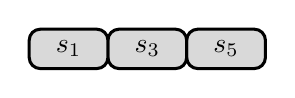
\begin{tikzpicture}[scale=0.5]
\heapblock{5}{1}{s_5};
\heapblock{3}{1}{s_3};
\heapblock{1}{1}{s_1};
\end{tikzpicture}
}
\subcaptionbox{\label{fig:convex subheap}}[.3\textwidth]{
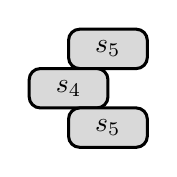
\begin{tikzpicture}[scale=0.5]
\heapblock{5}{3}{s_5};
\heapblock{4}{2}{s_4};
\heapblock{5}{1}{s_5};
\end{tikzpicture}
}
\subcaptionbox{\label{fig:saturated subheap}}[.3\textwidth]{
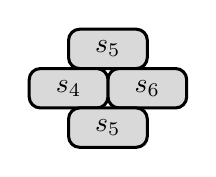
\begin{tikzpicture}[scale=0.5]
\heapblock{5}{3}{s_5};
\heapblock{6}{2}{s_6};
\heapblock{4}{2}{s_4};
\heapblock{5}{1}{s_5};
\end{tikzpicture}
}
\caption{Various subheaps of the heap in given in Figure~\ref{fig:first heap}.}
\label{fig:subheaps}
\end{figure}

From this point on, if there can be no confusion, we will not specify the exact subexpression that a subheap arises from.

The following fact is implicit in the literature (in particular, see the proof of~\cite[Proposition 3.3]{Stembridge1996}) and follows easily from the definitions.

%\begin{proposition}
%Let $(W,S)$ be a Coxeter system of type $\Gamma$ and let $w \in \FC(\Gamma)$. Then $H'$ is a convex subheap of $H(w)$ if and only if $H'$ is the heap for some subword of some reduced expression for $w$.   \qed
%\end{proposition}

%It will be extremely useful for us to be able to recognize when a heap corresponds to an element in $\FC(\C_{n})$.  The following lemma follows immediately from Remark~\ref{rem:illegal convex chains} and is also a special case of~\cite[Proposition 3.3]{Stembridge1996}.

%\begin{lemma}\label{lem:impermissible heap configs}
%Let $w \in \FC(\C_{n})$.  Then $H(w)$ cannot contain any of the following convex subheaps of Figure~\ref{fig:impermissible heap configs}, where $1<k<n+1$ and we use \begin{tabular}{c} 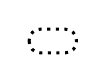
\begin{tikzpicture}[scale=0.3] \heapblank{0}{0}; \end{tikzpicture} \end{tabular} to emphasize that no element of the heap occupies the corresponding position.  \qed
%\end{lemma}

%\begin{figure}[!ht]
%\subcaptionbox{}[.3\linewidth]{
%\begin{tikzpicture}[scale=0.5]
%\heapblank{3}{3}
%\heapblock{2}{4}{s_2};
%\heapblock{1}{3}{s_1};
%\heapblock{2}{2}{s_2};
%\heapblock{1}{1}{s_1};
%\end{tikzpicture}
%}
%\subcaptionbox{}[.3\linewidth]{
%\begin{tikzpicture}[scale=0.5]
%\heapblank{3}{2}
%\heapblock{1}{4}{s_1};
%\heapblock{2}{3}{s_2};
%\heapblock{1}{2}{s_1};
%\heapblock{2}{1}{s_2};
%\end{tikzpicture}
%}
%\subcaptionbox{}[.3\linewidth]{
%\begin{tikzpicture}[scale=0.5]
%\heapblank{3}{2}
%\heapblock{2}{3}{s_{k+1}};
%\heapblock{1}{2}{s_k};
%\heapblock{2}{1}{s_{k+1}};
%\end{tikzpicture}
%}\\
%\vspace{1em}
%\subcaptionbox{}[.3\linewidth]{
%\begin{tikzpicture}[scale=0.5]
%\heapblank{0}{2}
%\heapblock{1}{3}{s_{k-1}};
%\heapblock{2}{2}{s_k};
%\heapblock{1}{1}{s_{k-1}};
%\end{tikzpicture}
%}
%\subcaptionbox{}[.3\linewidth]{
%\begin{tikzpicture}[scale=0.5]
%\heapblank{0}{2}
%\heapblock{2}{4}{s_{n+1}};
%\heapblock{1}{3}{s_n};
%\heapblock{2}{2}{s_{n+1}};
%\heapblock{1}{1}{s_n};
%\end{tikzpicture}
%}
%\subcaptionbox{}[.3\linewidth]{
%\begin{tikzpicture}[scale=0.5]
%\heapblank{0}{3}
%\heapblock{1}{4}{s_n};
%\heapblock{2}{3}{s_{n+1}};
%\heapblock{1}{2}{s_n};
%\heapblock{2}{1}{s_{n+1}};
%\end{tikzpicture}
%}
%\caption{Impermissible convex subheaps for elements in $\FC(\C_n)$.}%\label{fig:impermissible heap configs}
%\end{figure}

\end{subsection}
\end{section}
%%%%%%%%%%  Type A Stuff %%%%%%%%%%%%%
\begin{section}{Type $\A$ Stuff}

\begin{subsection}{Connection to Symmetric Group}
Some introductory sentence. Type $\A_n$ coxeter groups are isomorphic to the symmetric group on $n+1$ elements, $S_{n+1}$. We will not prove the isomorphism here but will give the relation between the two groups. It is known that all elements of the symmetric group can be written as adjacent 2-cycles. Given $s_i \in \A_n$ the corresponding element in $S_{n+1}$ is $(i, i+1)$ an adjacent 2-cycle. From this we see that $\A_n \cong S_{n+1}$ since $s_n=(n, n+1)$. Since this isomorphism exists we will use both Type $A_n$ and $S_{n+1}$ in the following sections for Type $A_n$. 
\end{subsection}

\begin{subsection}{String Diagrams}
Given the relation between Type $A_n$ and the symmetric group every reduced expression can be expressed as a string diagram that will allow us to visualize a reduced expression. It is important to note that the string diagram is not the string graph of $\A_n$ that is seen in Figure~\ref{fig:typeA}. Let $(W,S)$ be a Coxeter system of Type $A_n$. Suppose $\w=s_{x_1} \ldots s_{x_r}$ is a fixed reduced expression for $w \in W$. We see that $\w$ corresponds to the following element in $S_{n+1}$, $\sigma=(x_1,x_{x+1})(x_2,x_{x+2}) \ldots (x_r,x_{r+1})$, where $(x_i,x_{i+1})$ is the adjacent transposition defined above. We construct a string diagram as follows, create two columns of $n+1$ nodes that align node $1$ with node $1$ as the top most nodes, node $2$ with node $2$ as the second nodes in each column and so on ending with node $n+1$ aligned with node $n+1$ as the bottom most nodes. Now starting with node $1$ on the right utilize $\sigma$ to find where $1$ ends up, say $j$ and draw a line connection node $1$ on the right to node $j$ on the left. Repeat for nodes $2$ through $n+1$. \\
A \emph{crossing} in a string diagram refers to the location in which two strings cross. In Type $A_n$ two distinct strings will cross a maximum of one time. 
\begin{example}\label{ex:first string}
Let $\w=s_3 s_5 s_2 s_4 s_6 s_1 s_5 s_2$ be a reduced expression for $w \in W(\A_6)$. We see that $\w$ corresponds to the following element in $S_7$,~$\w=(34)(56)(23)(45)(67)(12)(56)(23)$. The labeled string diagram for $w$ is shown in Figure~\ref{fig:firststring}.

\begin{figure}
\begin{center}
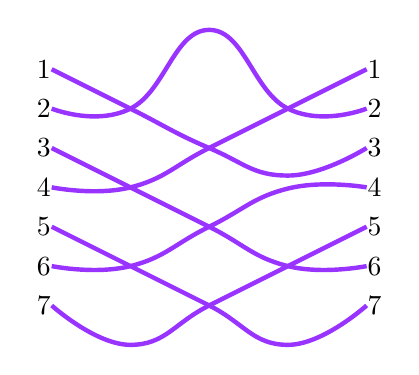
\begin{tikzpicture}[scale=0.5]
\node at (7.2,4) {$1$};
\node at (7.2,3) {$2$};
\node at (7.2,2) {$3$};
\node at (7.2,1) {$4$};
\node at (7.2,0) {$5$};
\node at (7.2,-1) {$6$};
\node at (7.2,-2) {$7$};

\node at (-1.2,4) {$1$};
\node at (-1.2,3) {$2$};
\node at (-1.2,2) {$3$};
\node at (-1.2,1) {$4$};
\node at (-1.2,0) {$5$};
\node at (-1.2,-1) {$6$};
\node at (-1.2,-2) {$7$};

\draw [purple,ultra thick] plot [smooth, tension=0.8] coordinates {(7,4)(5,3)(3,2)(1,1)(-1,1)};
\draw [purple,ultra thick] plot [smooth, tension=0.8] coordinates {(7,3)(5,3)(3,5)(1,3)(-1,3)};
\draw [purple,ultra thick] plot [smooth, tension=0.8] coordinates {(7,2)(5,1.3)(3,2)(1,3)(-1,4)};
\draw [purple,ultra thick] plot [smooth, tension=0.8] coordinates {(7,1)(5,.97)(3,0)(1,-1)(-1,-1)};
\draw [purple,ultra thick] plot [smooth, tension=0.8] coordinates {(7,0)(5,-1)(3,-2)(1,-3)(-1,-2)};
\draw [purple,ultra thick] plot [smooth, tension=0.8] coordinates {(7,-1)(5,-1)(3,0)(1,1)(-1,2)};
\draw [purple,ultra thick] plot [smooth, tension=0.8] coordinates {(7,-2)(5,-3)(3,-2)(1,-1)(-1,0)};
\end{tikzpicture}
\end{center}
\caption{NEEDS CAPTION.}\label{fig:firststring}
\end{figure}

In this case our string diagrams correspond to a left version of \cite{Jones.B:A} and several other papers. That is, in this paper the strings are moved from the right to the left as opposed to the top to the bottom in the corresponding reduced expression.
 
\end{example}
\end{subsection}

\begin{subsection}{Connection between String Diagrams and Heaps}
It is well-known folklore that heaps can be derived from string diagrams and string diagrams can be derived from heaps. We will first show how to construct a string diagram from a heap. Fix a reduced expression $\w=s_i\ldots s_r$ and construct the corresponding heap. For a heap block corresponding to a generator $s_n$ and label the node corresponding to the top of the block with $n$ and the node at the bottom of the block with $n+1$. In the center of the block create a square node which indicates a string crossing, wherever a block is missing place an x indicating. Repeat this for each block in the heap. Starting in the top most right node labeled with a 1 and trace the string to the closest square node or x, if the string hits a node it will pass through to the next node or x, if the string hits an x it will bounce in the opposite direction the string was traveling going towards the next node or x in the next column.
\begin{example}\label{ex:string to heap}
Let $\w=s_1 s_2 s_3 s_5$ be a a reduced expression for $w \in W(A_5)$. The heap is as follows from Example~\ref{ex:first heap}. Here we have labeled the top and bottom of the heaps appropriately, put the square nodes in the center of the heap blocks to nodes, put an X in the center of missing heap blocks, and overlaid the strings as well. 
\begin{center} 
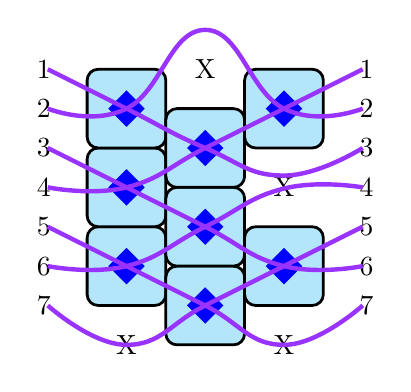
\begin{tikzpicture}[scale=0.5]
\nsq{0}{0}{};
\nsq{0}{2}{};
\nsq{0}{4}{};
\nsq{2}{-1}{};
\nsq{2}{1}{};
\nsq{2}{3}{};
\nsq{4}{0}{};
\nsq{4}{4}{};

\node at (7.1,4) {$1$};
\node at (7.1,3) {$2$};
\node at (7.1,2) {$3$};
\node at (7.1,1) {$4$};
\node at (7.1,0) {$5$};
\node at (7.1,-1) {$6$};
\node at (7.1,-2) {$7$};

\node at (-1.1,4) {$1$};
\node at (-1.1,3) {$2$};
\node at (-1.1,2) {$3$};
\node at (-1.1,1) {$4$};
\node at (-1.1,0) {$5$};
\node at (-1.1,-1) {$6$};
\node at (-1.1,-2) {$7$};

\node[diamond, fill=darkblue] at (5,3) {};
\node[diamond, fill=darkblue] at (5,-1) {};
\node[diamond, fill=darkblue] at (3,2) {};
\node[diamond, fill=darkblue] at (3,0) {};
\node[diamond, fill=darkblue] at (3,-2) {};
\node[diamond, fill=darkblue] at (1,3) {};
\node[diamond, fill=darkblue] at (1,1) {};
\node[diamond, fill=darkblue] at (1,-1) {};
\node at (5,1) {X};
\node at (3,4) {X};
\node at (1,-3) {X};
\node at (5,-3) {X};

\draw [purple,ultra thick] plot [smooth, tension=0.8] coordinates {(7,4)(5,3)(3,2)(1,1)(-1,1)};
\draw [purple,ultra thick] plot [smooth, tension=0.8] coordinates {(7,3)(5,3)(3,5)(1,3)(-1,3)};
\draw [purple,ultra thick] plot [smooth, tension=0.8] coordinates {(7,2)(5,1.3)(3,2)(1,3)(-1,4)};
\draw [purple,ultra thick] plot [smooth, tension=0.8] coordinates {(7,1)(5,.97)(3,0)(1,-1)(-1,-1)};
\draw [purple,ultra thick] plot [smooth, tension=0.8] coordinates {(7,0)(5,-1)(3,-2)(1,-3)(-1,-2)};
\draw [purple,ultra thick] plot [smooth, tension=0.8] coordinates {(7,-1)(5,-1)(3,0)(1,1)(-1,2)};
\draw [purple,ultra thick] plot [smooth, tension=0.8] coordinates {(7,-2)(5,-3)(3,-2)(1,-1)(-1,0)};
\end{tikzpicture}
\end{center}
\end{example}
This can be done to each heap to get the corresponding string diagram. This process can also be done to construct a heap from a string diagram. This is beyond the scope of this paper and will not be discussed here.\\
%Now we will show how to construct a heap from a string diagram. Given a string diagram for a reduced expression $\w$ create square nodes at each of the string crossings. Note that the squares fall precisely in the middle of two of the position nodes that we used to create the string diagram. Each of these square nodes corresponds to a unique heap element, if a square falls between $i,~i+1$ then the corresponding heap element has label $s_i$. 
%\begin{example}\label{ex:string to heap}
%Let $\w=s_1 s_2 s_3 s_5$ be a a reduced expression for $w \in W(A_5)$. The string diagram is as follows from Example~\ref{ex:first string}.\\
%
%\begin{figure*}
%	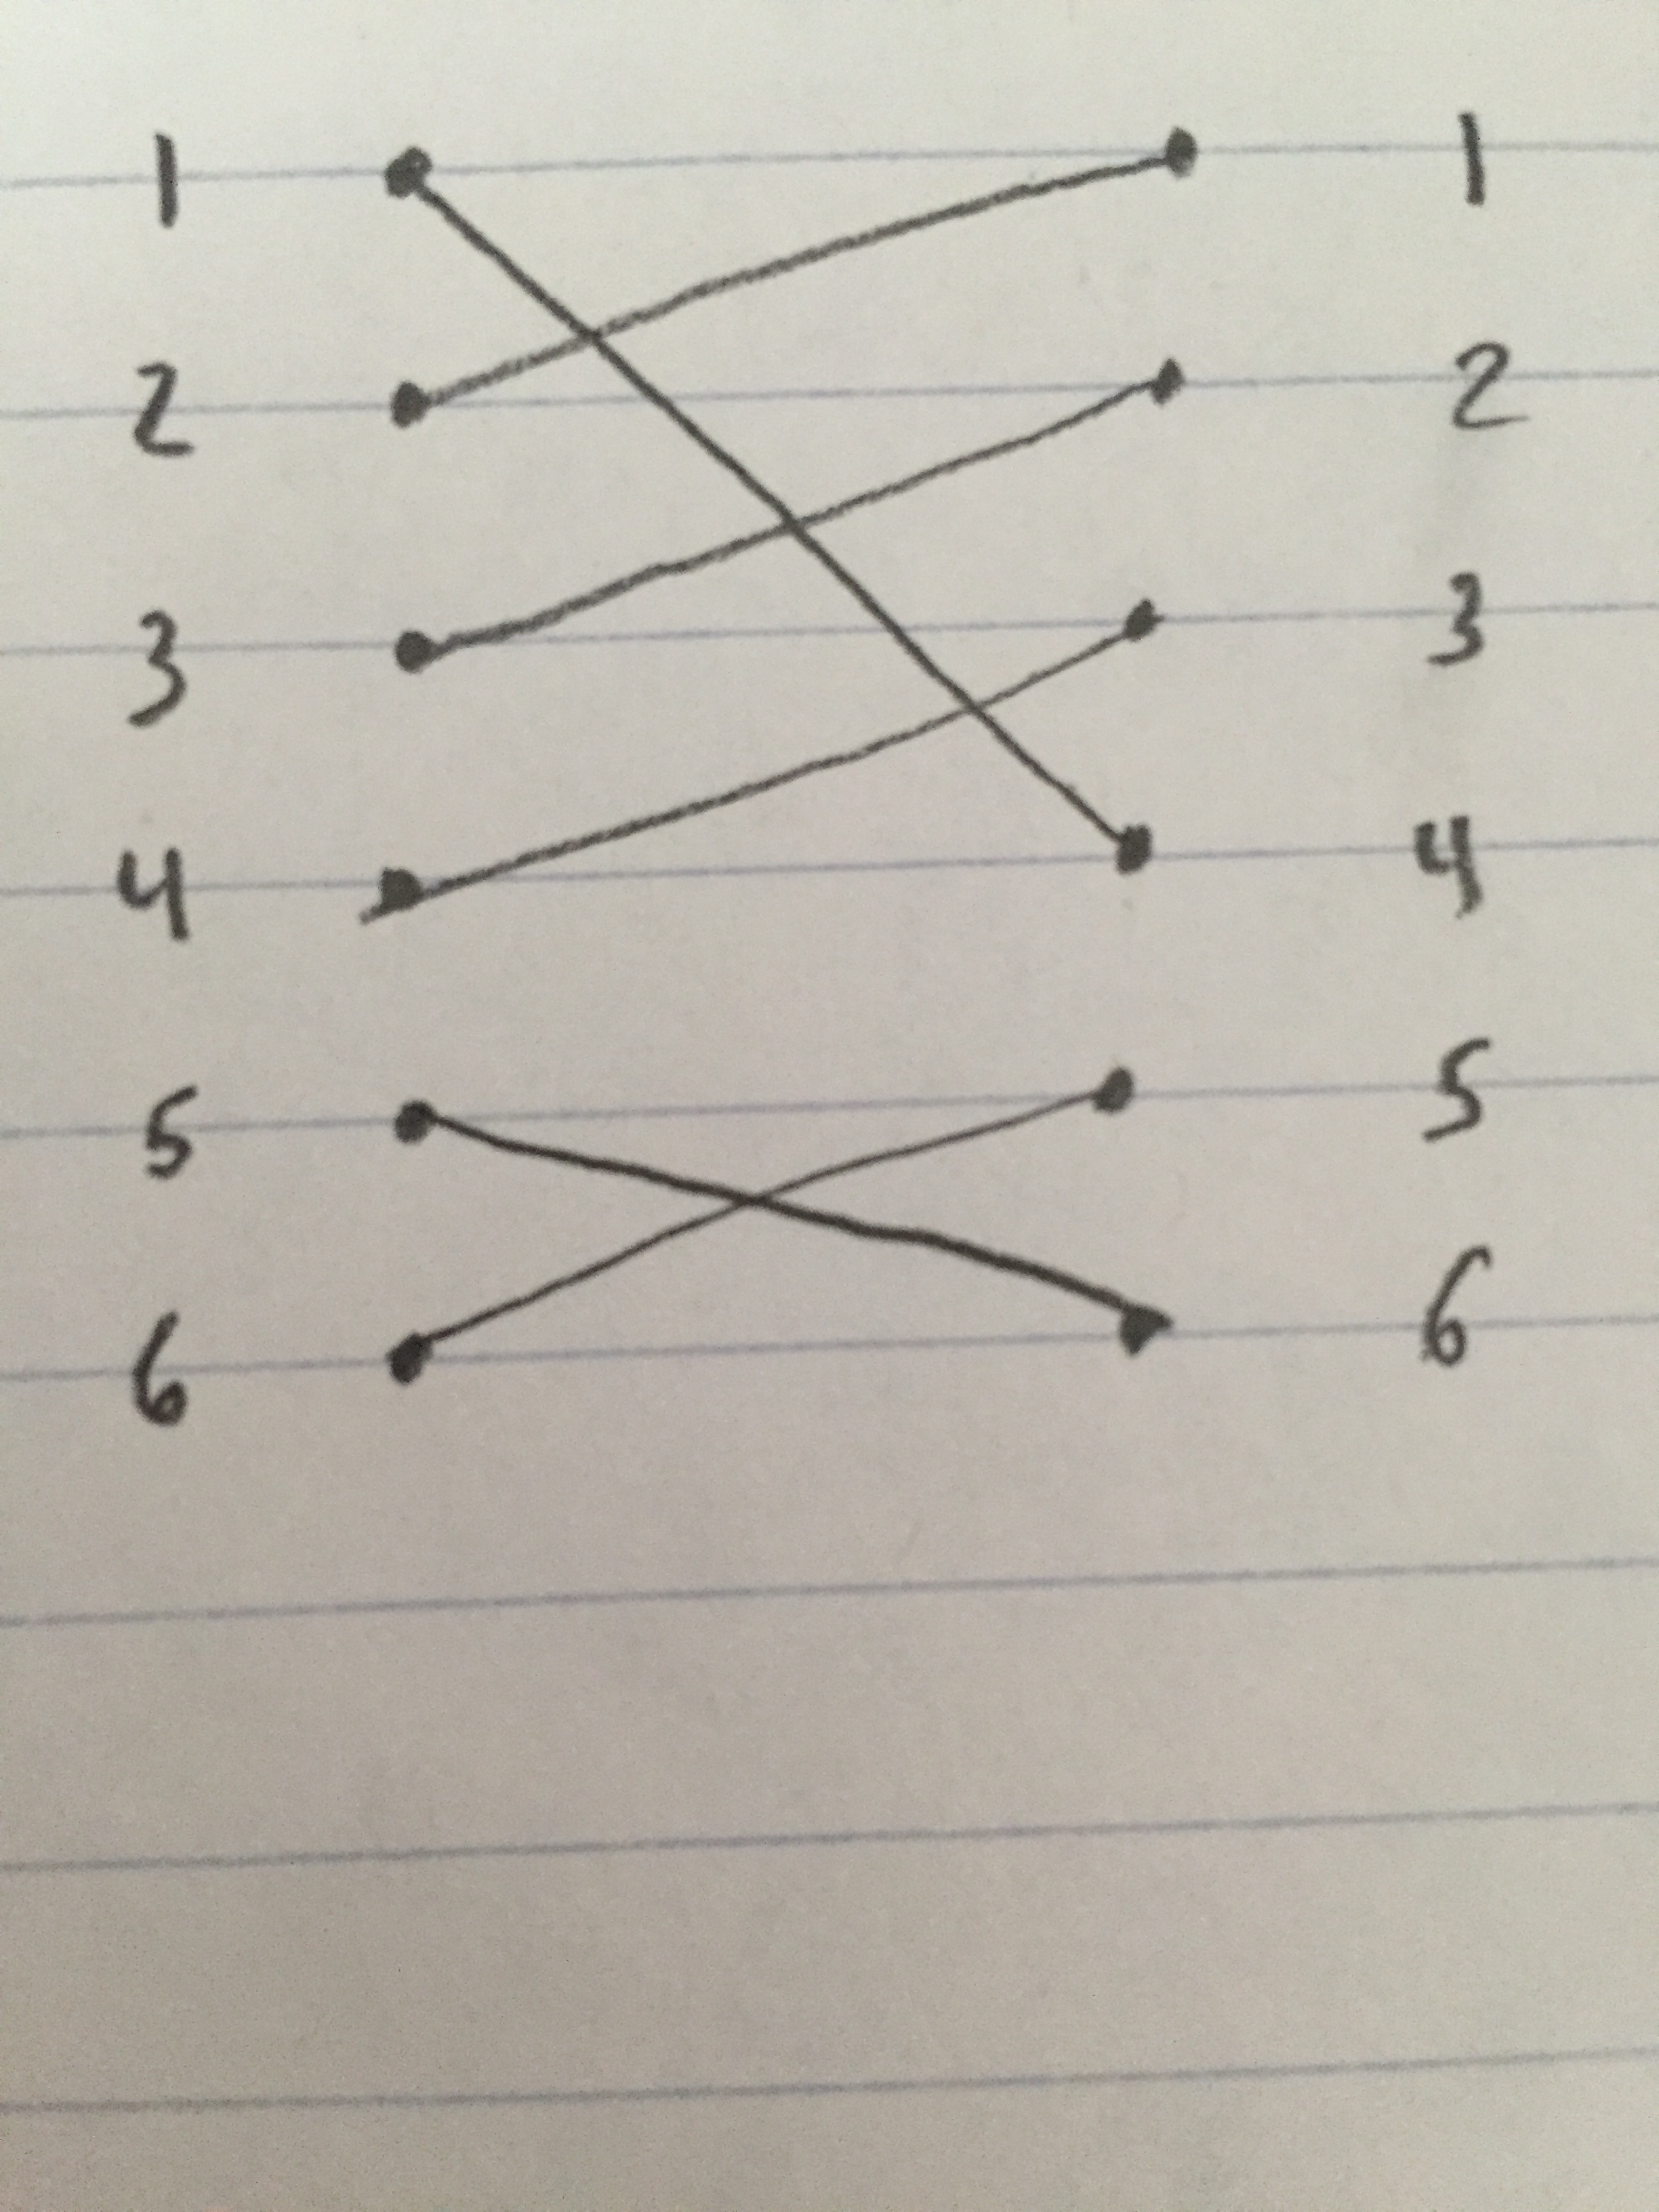
\includegraphics[scale=.05]{firststring.jpg}
%\end{figure*}
%\pagebreak
%At each of the string crossings we have created a square node. We see that the first square node on the left falls between position nodes $1$ and $2$, thus the corresponding heap element has label $s_1$. The second square node from the left falls between position nodes $2$ and $3$ and thus the corresponding heap element has label $s_2$. Continuing in this matter we get the following heap.\\
%
%\begin{figure*}
%	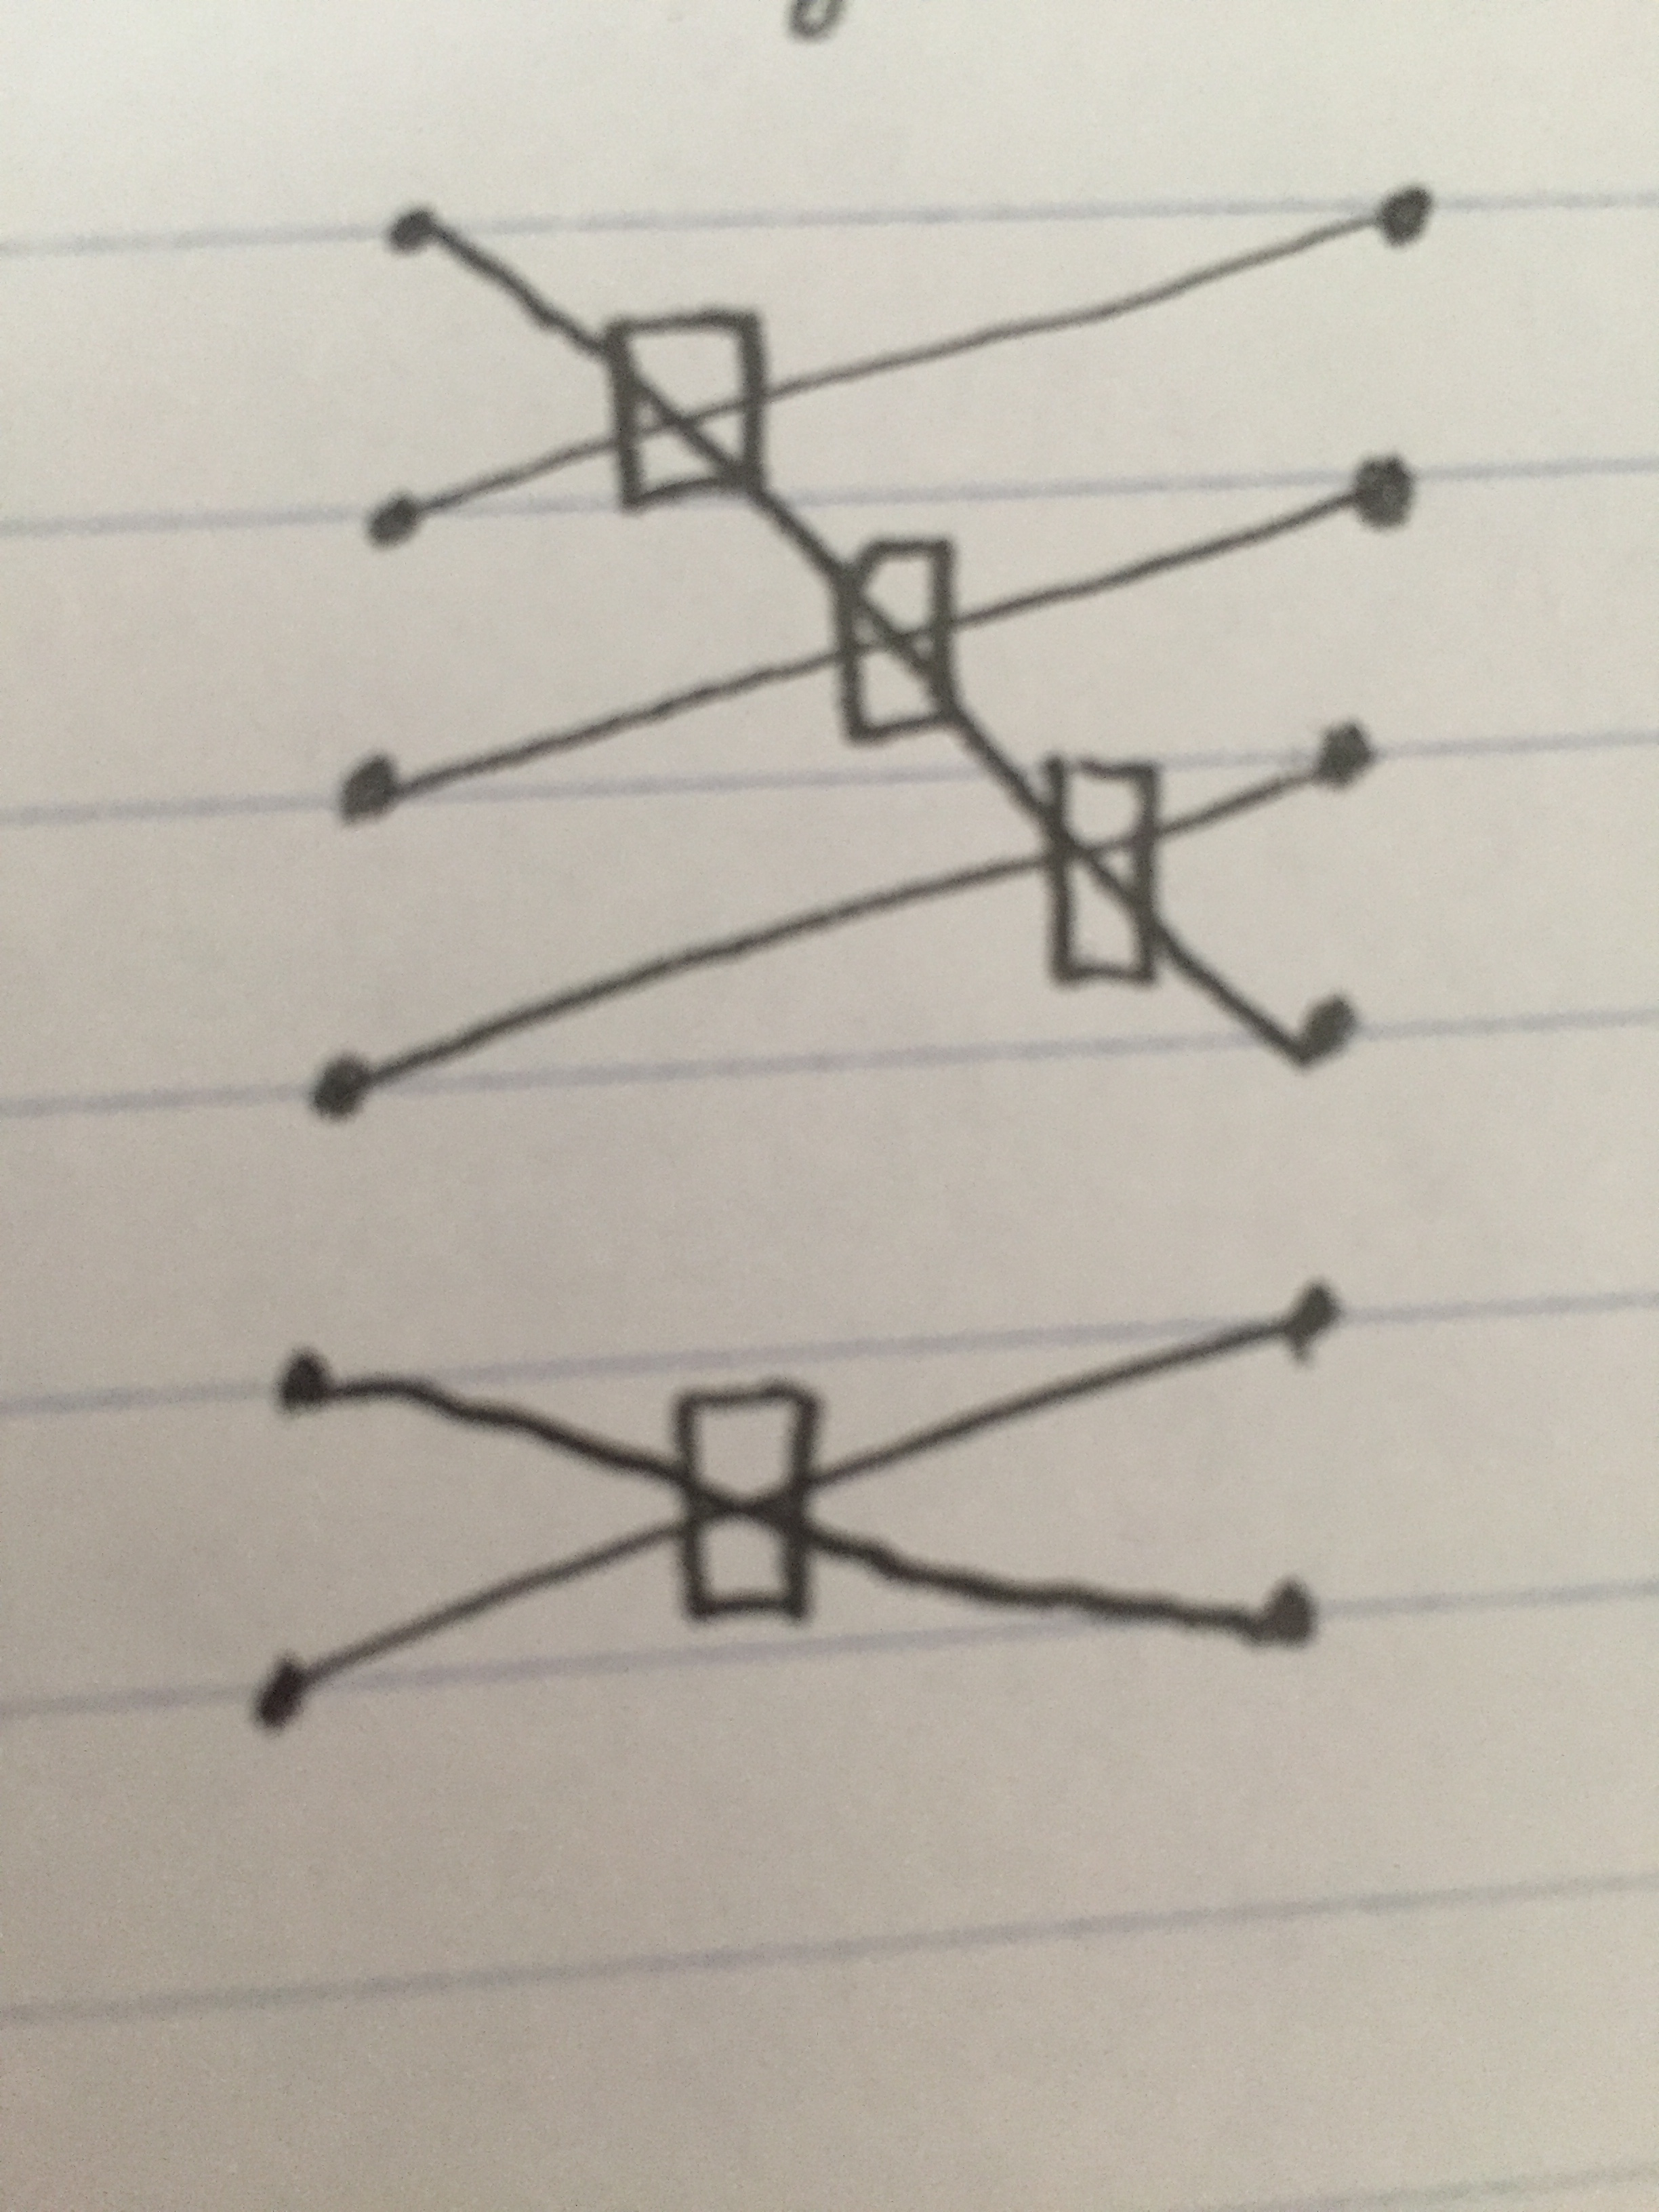
\includegraphics[scale=0.05]{stringtoheap.jpg}
%	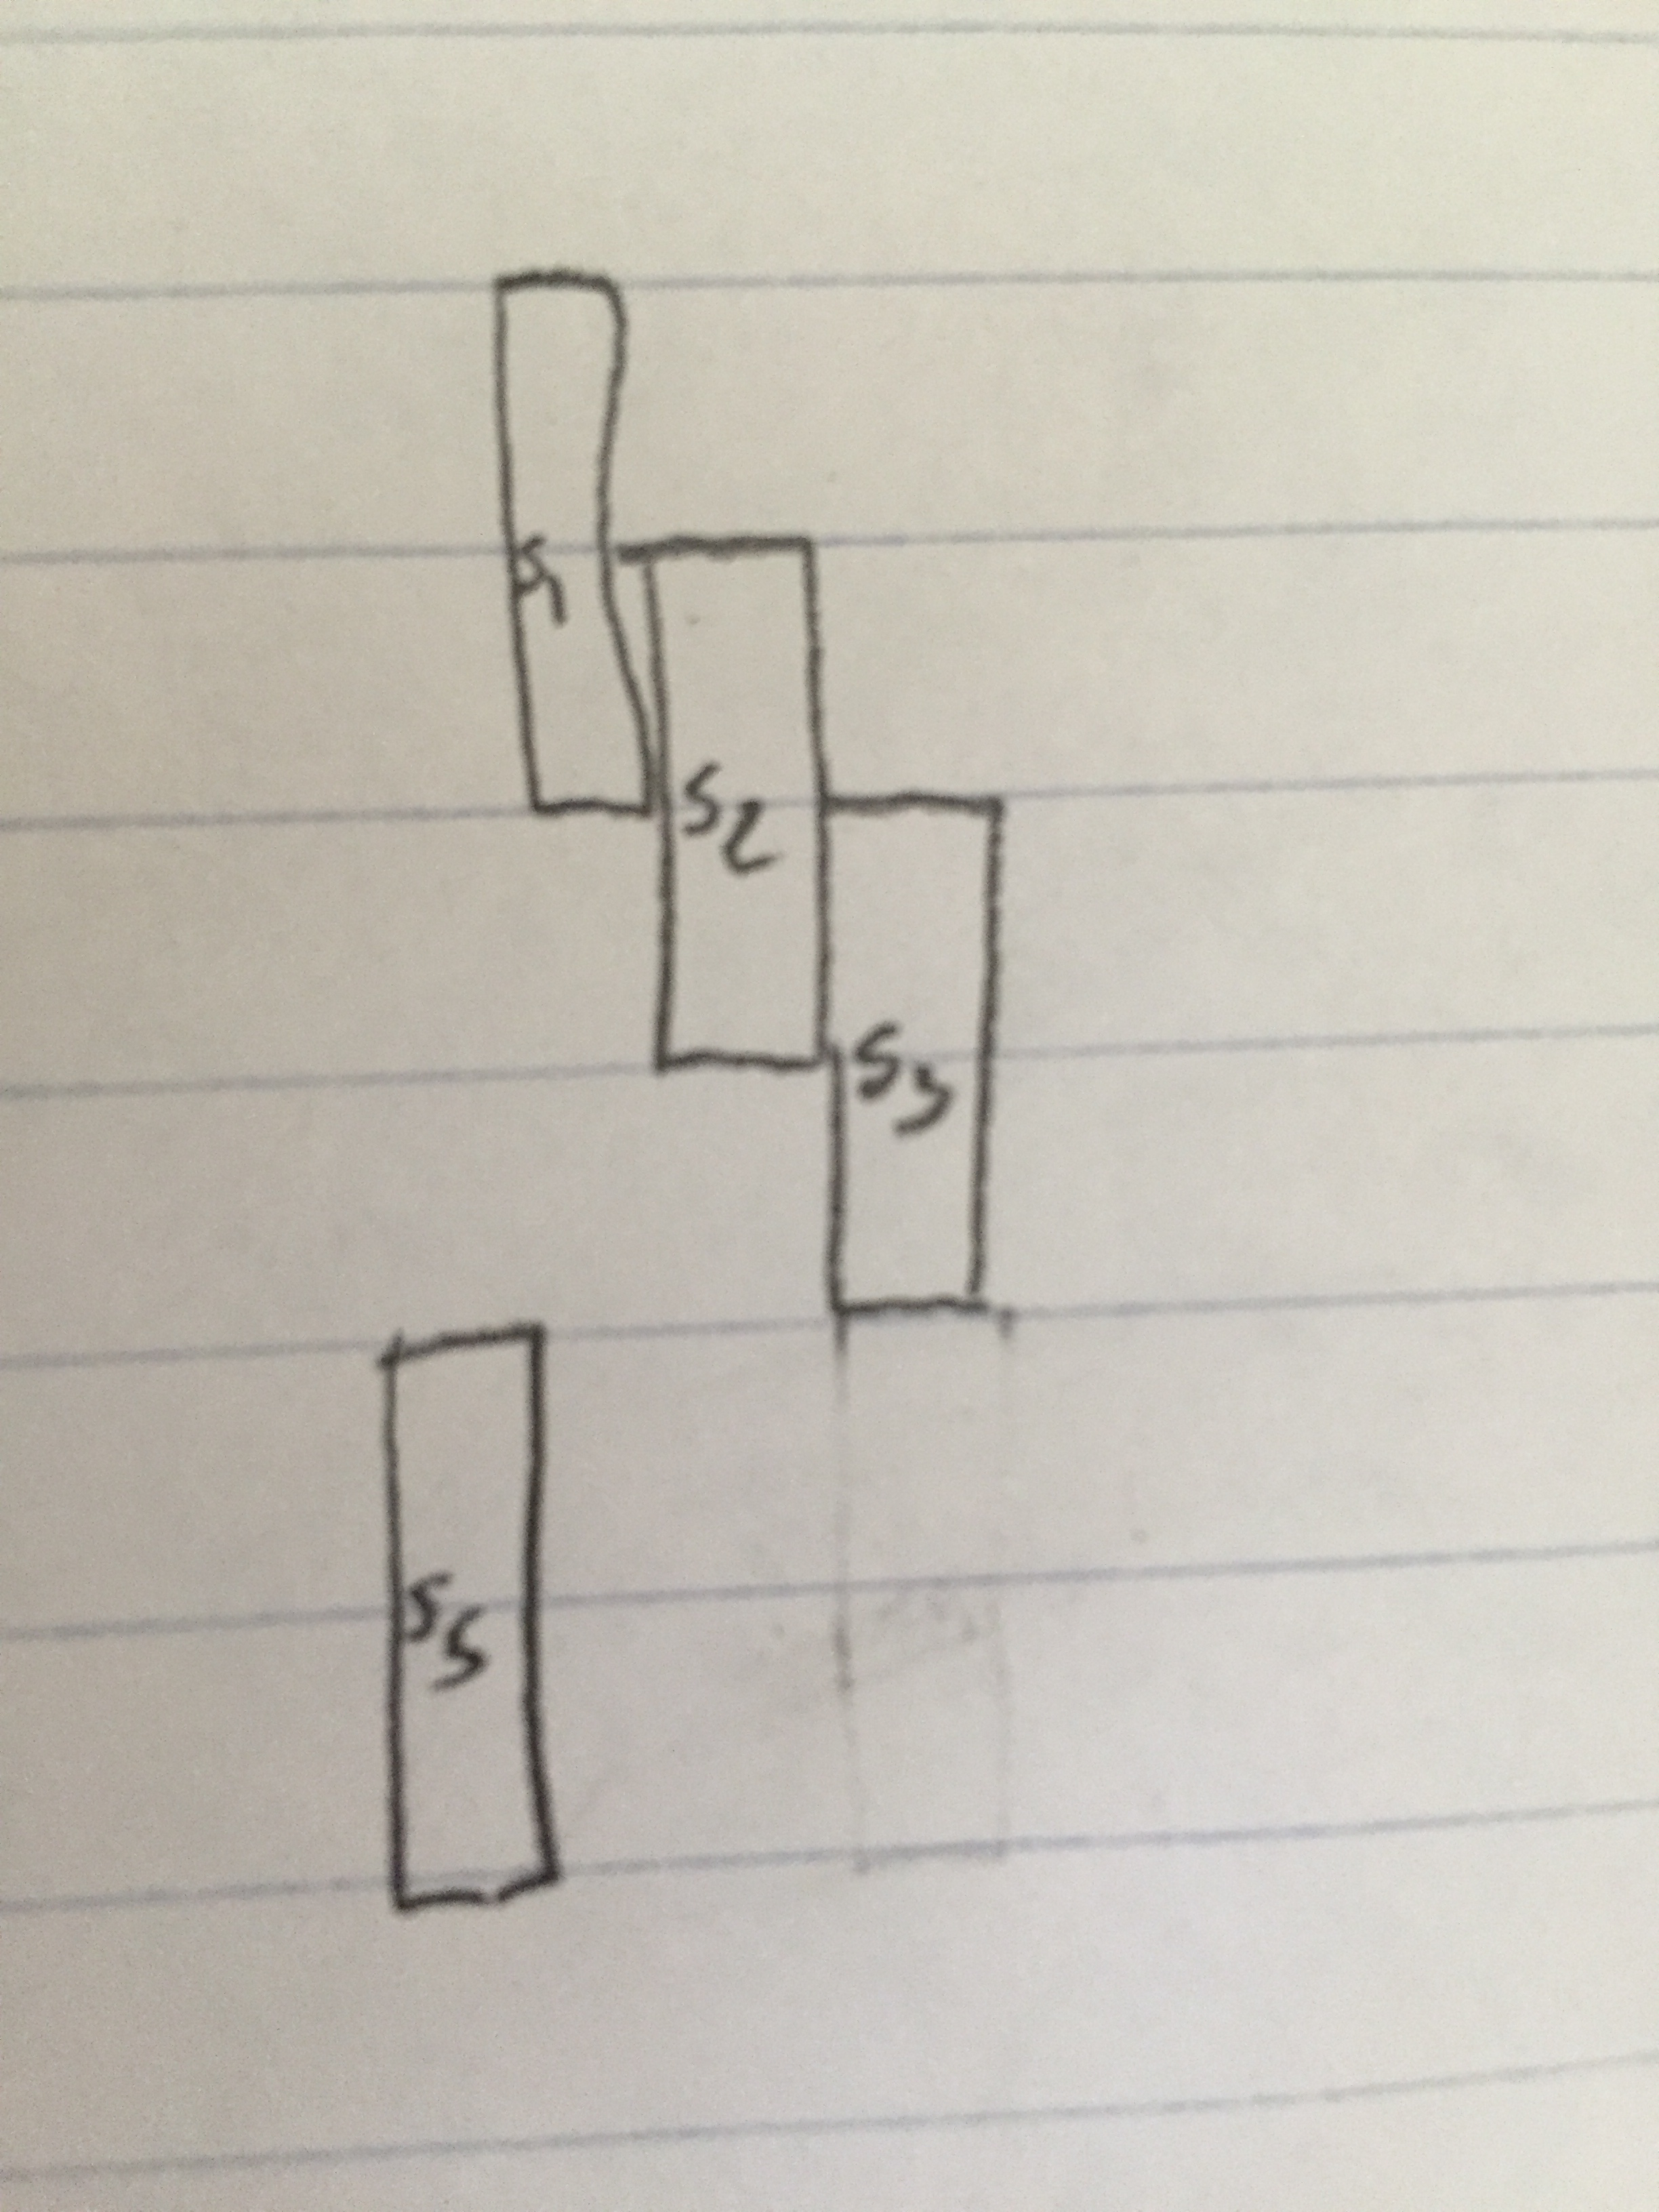
\includegraphics[scale=0.05]{stringheap}
%\end{figure*}
% 	
%\end{example}

\end{subsection}
\end{section}

%%%%%%%%%%  T-Avoiding in Type $A$ %%%%%%%%%%%%%
\begin{section}{T-Avoiding in Type A}
\begin{subsection}{Property T}
Given the connection to they symmetric groups of Type $(\A_n)$ we will consider the following definitions in terms of permutations in $S_{n+1}$. A permutation $\sigma \in S_{n+1}$ has \emph{Property T} if and only if there exists an $i$ such that either $\sigma(i)>\sigma(i+1), \sigma(i+2)$ or $\sigma(i+2)<\sigma(i),\sigma(i+1)$ Visually we see this in a string diagram as follows.~{\color{red} Insert property T pictures for Type A here} It is important to note that $\sigma$ containing Property T is not exclusive itself, if $\sigma^{-1}$ contains the same properties, then the element is said to have Property T.
\begin{example}
Consider $\sigma=(124)(35)$ in $S_{n+1}$. The string diagram for $\sigma$ is as follows. {\color{red} Insert String Diagram here with Property T marked off on the sides}. Note that $\sigma$ has Property T twice and $\sigma^{-1}$ has Property T once.	
\end{example}
\end{subsection}

\begin{subsection}{T-Avoiding and Bad Elements}
The focus of our research has been to find elements that don't contain Property T. An element $\sigma \in S_{n+1}$ is said to be \emph{T-avoiding} if and only if neither $\sigma$ nor $\sigma^{-1}$ have property T.	It is clear that if $\sigma$ is a product of commuting adjacent 2 cycles then $\sigma$ is T-avoiding. When $\sigma$ is an element of $S_n$ of this type we say that $\sigma$ is \emph{trivially T-avoiding}. An element $\sigma \in S_{n+1}$ that is T-avoiding by not trivially T-avoiding is called \emph{bad}. 
\end{subsection}

\begin{subsection}{T-Avoiding in Type \textbf{$A_n$}}
We will show that there are no bad elements in Type $A_n$. To do this we will show that there are no bad elements in $S_n$ since they are isomorphic.
\begin{proposition}
Elements in $S_n$ are T-Avoiding if and only if the elements are products of commuting adjacent 2 cycles.
\end{proposition}
\begin{proof}
$(\Leftarrow)$ Let $\sigma$ be a product of commuting adjacent 2 cycles. Then $\sigma$ is trivially T-avoiding.\\
$(\Rightarrow)$ To show this direction we will show the contrapositive is true. That is \emph{if $\sigma$ is not the product of commuting adjacent 2-cycles then either $\sigma$ or $\sigma^{-1}$ has Property T}. Assume that $\sigma$ is not a product of commuting adjacent 2-cycles. This implies that any heap for $\sigma$ has at least 2 columns and that the string diagram has at least one string with more than one crossing. We will proceed in two cases which we will call the easy case and the hard case. \\
\textbf{Easy case} There is at least one node in the second column (left or right hand side) is blocked by only one other node. Without loss of generality suppose the $i+1^{st}$ node is blocked in the $i^{th}$ position but not in the $i+2^{nd}$ position. Then $\sigma(i) \geq i+1$, but $\sigma(i+1) \leq i$ and $\sigma(i+2) \leq i$. {\color{red} picture of the case}. Thus $\sigma$ has Property T.\\
\textbf{Hard case} Every node in the second column (left or right hand side) is blocked by 2 nodes in the first column, however somewhere in the heap there exists nodes in the $i-1^{st}$ column in the $\i^{th}$ position, in the $i^{th}$ column in the $i-1^{st}$ or in the $i+1^{st}$ position, and in the $i+1^{st}$ column in the $i^{th}$ position. {\color{red} picture of the pattern we are looking for}. Without loss of generality we will look at this case from the right hand side which implies that our first column referred to later is the right most column and continuing numbering in the left direction columns. First, we will show that if we are in the hard case then $\sigma$ is not fully commutative. For the sake of contradiction suppose $\sigma$ is fully commutative and minimal, then there is only one heap corresponding to $\sigma$ which has 3 or more columns. Because we are in the hard case, every node in the second column is blocked by two nodes in the first column. Delete the first column. We should be left with an element that is FC. However, since we chose a minimal case deleting the first column creates an element in the easy case. Because of this we see that $\sigma$ can not be FC. This implies that $\sigma$ contains the diamond shape we are looking for. Since we now know that the diamond shape exists in $\sigma$ it is easy to see that we have one of the following pictures occur within the string diagram of $\sigma$. {\color{red} Picture of the cases}. Thus, $\sigma$ has Property T.\\
Therefore, if $\sigma$ is not the product of commuting adjacent 2-cycles, then either $\sigma$ or $\sigma^{-1}$ has Property T and elements in $S_n$ are T-Avoiding if and only if the elements are products of commuting 2-cycles.   
\end{proof}

\end{subsection}	
\end{section}

%%%%%%%%%%%%%%%%%%%%%%%%%%%%%%%%%Type B_n%%%%%%%%%%%%%%%%%%%%%%%%%%%%%%%%%%%%

\begin{section}{Type $B_n$}
	\begin{subsection}{Diagonal Factorization}
		Some sort of introductory sentence. To start with we will define the following sets, $w^{(0)}=\{e, s_0\}$, $w^{(1)}=\{e, s_1, s_1s_0, s_1s_0s_1\}$, $w^{(2)}=\{e, s_2, s_2s_1, s_2s_1s_0, s_2s_1s_0s_1, s_2s_1s_0s_1s_2\}$ and $w^{(i)}=\{e, s_i, s_is_{i-1}, \ldots, s_is_{i-1}\ldots s_1s_0, \ldots, s_1s_{i-1}\ldots s_1s_0s_1 \ldots s_{i-1}s_i\}$. It was shown in {\color{red} paper name}, that if $w \in W(B_n)$, then $w$ can be written in the following way $w=w_0w_1w_2\ldots w_n$, where each $w_i \in W^{(i)}$. 
	\end{subsection}
\end{section}

\begin{section}{T-Avoiding in Type B}
\begin{subsection}{Property T}
A slightly different definition is required for Property T for Type $B_n$, as we no longer have the close connection the symmetric group. Suppose $w \in B_n$, then $w$ has Property T if and only if $w=stu$ or $w=uts$ is reduced and $m(s,t) \geq 3$, and $u \in B_n$. 	
\end{subsection}


\begin{subsection}{T-Avoiding in Type $B_n$}
In the following section we will show that there are no bad elements in type $B_n$. In order to do this we first will prove several lemmas, and then we will prove the theorem. In the following, unless otherwise stated $w$ is presented in the diagonal factorization.
\begin{lemma}
If $w_n=s_n$, $w_{n-1}=s_{n-1}s_{n-2}$ and $w_i=e$ for all $i \neq n, n-1$, then $w$ has Property T on the left.	
\end{lemma}
\begin{proof}	
Suppose $w_n=s_n$, $w_{n-1}=s_{n-1}s_{n-2}$ and $w_i=e$. Then $w=s_{n-1}s_{n-2}s_n$. Clearly $w$ has Property T on the left.
\end{proof}

\begin{lemma}
If everything in the second column (on the right) is blocked by two things in the rightmost column in the heap of $w$ and all the zigs attain maximum height, then $w$ has Property T on the left.	Here maximum height is defined to be the block in the rightmost column, or $s_0$ if it does not reach the right most column.
\end{lemma}
\begin{proof}
Suppose everything in the second column is blocked by two things in the rightmost column in the heap of $w$, and all zigs attain maximum height. Then $w=s_0s_1s_0s_2s_1s_0w_3 \ldots w_n$, and clearly $w$ has Property T on the left.	
\end{proof}

\begin{lemma}
If everything in the second column is blocked by two things in the rightmost column, and not all $w_k$ attain maximum height as defined above,then $w$ has Property T on the right.
\end{lemma}
\begin{proof}
Suppose that everything in the second column of the heap of $w$ is blocked by two things in the rightmost column of $w$. Choose the maximal $k$ such that $w_k$ does not attain maximum height. We proceed in the following cases.
	\begin{itemize}
	\item Case 1: The $w_k$ 	that does not attain maximum height is one which would contribute to the rightmost column.\\
		Suppose that the maximal $k$ such that $w_k$ does not attain maximal height is one which would contribute to the rightmost column of the heap. Then we can write $w_k=s_ks_{k-1} \ldots s_i$ and we can write $w=w_0 \ldots w_{k-1} s_k s_{k-1} \ldots s_i s_{k+1} s_k \ldots s_j w_{k+1} \ldots w_n$. Note that $s_j$ is in the right most column.\\
		 If $s_i=s_j$, then applying commutations to $w$ we see that $w=w_0 \ldots w_{k-1} s_k s_{k-1} \ldots s_{i-1} s_{k+1} s_k \ldots s_i s_{j+1} s_j w_{k+1} \ldots w_n$. Applying a braid to the $s_i s_{j+1} s_j$ elements we get that $w=w_0 \ldots w_{k-1} s_k s_{k-1} \ldots s_{i-1} s_{k+1} s_k \ldots s_{j+1} s_{j} s_{j+1} w_{k+1} \ldots w_n$. In applying the braid move to $w$ we have created a gap in the rightmost wall of the heap. Because of this gap we can apply commutations to $w$ and $w=w_0 \ldots w_{k-1} s_k s_{k-1} \ldots s_{i-1} s_{k+1} s_k \ldots s_{j+1} w_{k+1} \ldots w_n s_{j+1} s_{j}$ and thus $w$ has Property T on the right.\\
		 Now consider $s_i \neq s_j$. Since $w_{k+1}$ attains maximum height $s_i \in \Sup(w_{k+1})$. Then by applying commutations to $w$ above we see that $w=w_0 \ldots w_{k-1} s_k s_{k-1} \ldots s_{i-1} s_{k+1} s_k \ldots s_i s_{i+1} s_i \ldots s_j w_{k+1} \ldots w_n$. Using the braid moves described at the end of the Type $\A$ proof, which is legal since except for $s_0, s_1$ the same relations hold, we can using braid moves the $s_i s_{i+1} s_i$ to the rightmost wall. In doing this we have created a gap in the rightmost column and by applying the same commutations from above we see that $w=w_0 \ldots w_{k-1} s_k s_{k-1} \ldots s_{i-1} s_{k+1} s_k \ldots s_{j+1} w_{k+1} \ldots w_n s_{i+1} s_{i}$, which has Property T on the right. 
	\item The $w_k$ that does not attain maximum height is not one which would contribute to the right most column.\\
		Suppose that the maximal $k$ such that $w_k$ does not attain maximal height is not one which would contribute to the rightmost column. Since $w_k$ does not attain maximal height we can write $w_k=s_k \ldots s_i$ where $s_i \neq 0$. However, since $w_{k+1}$ attains maximal height $s_i \in \Sup(w_{k+1})$. Then we can write $w=w_0 \ldots w_{k-1} s_k s_{k-1} \ldots s_i s_{k+1} s_k \ldots s_i \ldots s_j w_{k+1} \ldots w_n$. By applying commutations we see that  $w=w_0 \ldots w_{k-1} s_k s_{k-1} \ldots s_{i-1} s_{k+1} s_k \ldots s_i s_{i+1} s_i \ldots s_j w_{k+1} \ldots w_n$. Then as above we can apply braid moves to $s_i s_{i+1} s_i$ to create a gap in the rightmost column and applying the commutations as above we get $w=w_0 \ldots w_{k-1} s_k s_{k-1} \ldots s_{i-1} s_{k+1} s_k \ldots s_{j+1} w_{k+1} \ldots w_n s_{i+1} s_{i}$. Thus $w$ has Property T on the right.
	\end{itemize}
Therefore, if everything in the second column is blocked by two things in the rightmost column, and not all $w_k$ attain maximum height as defined above,then $w$ has Property T on the right.
\end{proof}

The above lemmas when combined together show that if the elements in the second column of the heap of $w$ are blocked by two things in the first column then $w$ has Property T. We will use this fact in the proof the following proof.

\begin{theorem}
	In Type $B_n$, elements, $w \in B_n$, are T-Avoiding if and only if $w$ is a product of commuting generators.
\end{theorem}

\begin{proof}
	Let $w \in B_n$ be a reduced expression with diagonal factorization.\\
	$(\Leftarrow)$ Suppose $w$ is a product of commuting generators. Then $w$ is trivially $T-Avoiding$.\\
	$(\Rightarrow)$ To prove this direction we will show the contrapositive. That is, if $w$ is not a product of commuting generators then $w$ has Property T on the left or right.\\
	Suppose $w$ is not a product of commuting generators. If $s_0$ is not in the support of $w$, then $w$ is a Type $\A_{n-1}$ element and we are done. Consider $s_0 \in \Sup(w)$. Since $w$ is not a product of commuting generators there exists a maximal $k$ such that $w_k \neq \{e, s_k\}$. That is, $w_k=s_k \ldots s_i$ for $i \in \{1, \ldots ,k-1\}$. The rest proceeds in case analysis.
	\begin{enumerate}
	\item The minimal $k=n$
	\begin{enumerate}
	\item Suppose $w_n=s_ns_{n-1} \ldots s_i$ for $i \in \{0, \ldots ,n-1\}$ and $w_n$ does not zig-zag. Then $w=w_0 \ldots w_{k-1} s_n s_{n-1} \ldots s_{i+1} s_i$, which implies that $w$ has Property T on the right.
	\item Suppose $w_n=s_n s_{n-1} \ldots s_i$ for $i \in \{0, \ldots ,n\}$ and $w_n$ does zig-zag. Then $w=w_0 \ldots w_{n-1} s_n s_{n-1} \ldots s_1 s_0 s_1 \ldots s_i$, which implies $w$ has Property T on the right.
	\end{enumerate}
	\item The minimal $k < n$.
	\begin{enumerate}
	\item The element $w_{k+1}=e$.
	\begin{enumerate}
	\item Suppose $w_k =s_k \ldots s_i$ for $i \in \{1, \ldots k-1\}$ and $w$ does not zig zag. Then $w=w_0 w_1 \ldots w_{k-1} s_k \ldots s_i e w_{k+2} \ldots w_n$ which when commutations are applied to $w$ we see that $w=w_0 w_1 \ldots w_{k-1} e w_{k+2} \ldots w_n s_k \ldots s_i$. This shows that $w$ has Property T on the right.
	\item Suppose $w_k=s_k \ldots s_i$ for $s_i \in \{0, k\}$. and $w$ zig zags. then $w=w_0 \ldots w_k-1 s_k s_{k-1} \ldots s_i e w_k+2 \ldots w_n$ which applying commutations, a possibility since for $i \geq k+1$, $w_i$ is either $e$ or $s_i$, gives $w=w_0 \ldots w_{k-1} s_k \ldots s_{i-2} w_{k+1} \ldots w_n s_{i-1} s_i$ which clearly has Property on the right.
	\end{enumerate}
	\item The element $w_{k+1} \neq e$.
	\begin{enumerate}
	\item Suppose $w_k=s_k \ldots s_i$ for $i \in \{0, \ldots k\}$ and $w$ zig-zags, and write $w=w_0 \ldots w_{k-1} s_k \ldots s_i w_{k+1} \ldots w_n$.
	\begin{enumerate}
	\item Suppose $i=k$. Then we can write $w=w_0 \ldots w_{k-1} s_k \ldots s_1 s_0 s_1 \ldots s_k w_{k+1} \ldots w_n$.
	\begin{itemize}
	\item Suppose $w_{k+2}=e$.Then $w=w_0 w_{k-1} s_k \ldots s_1 s_0 s_1 \ldots s_k s_{k+1} e w_{k+3} \ldots w_n$ which after applying commutations $w=w_0 w_{k-1} s_k \ldots s_1 s_0 s_1 \ldots s_k s_{k+1} e w_{k+3} \ldots w_n s_k s_{k+1}$. Thus $w$ has Property T on the right.
	\item Suppose $w_{k+2} \neq e$. Then $w=w_0 \ldots w_{k-1} s_k \ldots s_1 s_0 s_1 \ldots s_k s_{k+1} s_{k+2} w_{k+3} \ldots w_n$. If $w_{k+3}=e$ we are done as we can commute $s_{k+1}s_{k+2}$, which implies $w$ has Property T on the right. If $w_{k+3} \neq e$ and $w_{k+4} = e$, then we are done as we can commute $s_{k+2} s_{k+3}$ out to the right. Inductively, choose $w_{k+i}$ and $w_{k+1+i}$  such that neither is the identity and $w_{k+i+2}$ is the identity, and commute them out making $w$ have Property T on the right.
	\end{itemize}
	\item Suppose $i \neq k$. Then $w=w_0 \ldots w_{k-1} s_{k} \ldots s_1 s_0 s_1 \ldots s_{i+2} w_{k+1} \ldots w_n$. By applying commutations we see that $w=w_0 \ldots w_{k-1} s_k \ldots s_1 s_0 s_1 \ldots s_{i-2} w_{k+1} \ldots w_n s_{i+1} s_1$. Thus $w$ contains property Property T.
	\end{enumerate}
	\item Suppose $w_k=s_k \ldots s_i$ for $i \in \{0, \ldots, k-1\}$ and $w$ does not have zig zags.
	\begin{itemize}
	\item Suppose $i \neq k-1$. Then $w=w_0 \ldots w_{k-1} s_k \ldots s_i w_{k+1} \ldots w_n$. By apply commutations we see that $w=w_0 \ldots s_k \ldots s_{i+2} w_{k+1} \ldots w_n s_{i+1} s_i$. This implies that $w$ has Property T on the right.
	\item Suppose $s_i =s_{k-1}$. Then by the combinations of the lemmas we are done. 	
	\end{itemize}
	\end{enumerate}
	\end{enumerate}
	\end{enumerate}
	Therefore, in Type $B_n$ elements are T-Avoiding if and only if they are a product of commuting generators.
\end{proof}
\end{subsection}

	
\end{section}


\bibliographystyle{plain}
\bibliography{T-Avoiding}

\end{document}